\begin{center}
	\textbf{{\Huge ĐỀ 003}}
\end{center}
\subsubsection*{Phần I. Thí sinh trả lời từ câu 1 đến câu 12, mỗi câu hỏi chọn một phương án.}
\setcounter{bt}{0}\setlist[enumerate,1]{label=\quad\bfseries\Alph*.}
\begin{baitap}
	%	\textbf{Câu 1.} 
	Tìm giá trị nhỏ nhất của hàm số $y = \dfrac{x + 3}{x - 1}$ trên đoạn $[-1;0]$.
	\begin{multicols}{4}
		\begin{enumerate}
			\item $\min\limits_{[-1;0]} y = -3$.
			\item $\min\limits_{[-1;0]} y = -2$.
			\item $\min\limits_{[-1;0]} y = -4$.
			\item $\min\limits_{[-1;0]} y = 3$.
		\end{enumerate}
	\end{multicols}
	\begin{traloi}
		\dapan{A}
		Chỉ ra hàm số nghịch biến trên $ [-1;0] $ nên $ \min\limits_{[-1;0]} y=y(0)= -3.$
	\end{traloi}
\end{baitap}

\begin{baitap}
	%	\textbf{Câu 2.} 
	Cho hàm số $ y=f(x) $ có đồ thị như hình vẽ sau. Giá trị nhỏ nhất trên tập xác định $ \mathcal{D} $ của hàm số là
	
	\begin{minipage}{0.4\textwidth}
		\begin{enumerate}
			\item $\min\limits_{\mathcal{D}} y = -1$.
			\item $\min\limits_{\mathcal{D}} y = 1$.
			\item $\min\limits_{\mathcal{D}} y = 0$.
			\item $\min\limits_{\mathcal{D}} y = -2$.
		\end{enumerate}
	\end{minipage}
	\begin{minipage}{0.4\textwidth}
		% Biquadratic function y = x^4 - 2x^2 with local max at (0,0) and local mins at (-1,-1) and (1,-1)
		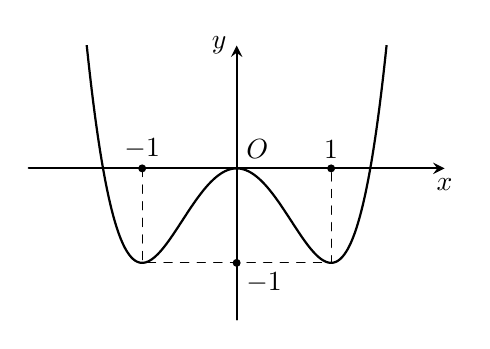
\begin{tikzpicture}[line cap=round, line join=round, >=stealth, scale=1.2]
			% Define window bounds
			\def\xmin{-2.2} \def\xmax{2.2}
			\def\ymin{-1.6} \def\ymax{1.3}
			
			% Scope to clip the polynomial curve within bounding box
			\begin{scope}
				\clip (\xmin,\ymin) rectangle (\xmax,\ymax);
				
				% Graph of y = x^4 - 2x^2
				\draw[black, thick, smooth, samples=200, domain=\xmin:\xmax]
				plot(\x, {(\x)^4 - 2*(\x)^2});
			\end{scope}
			
			% Dashed projection lines connecting local minima (-1,-1) and (1,-1) to axes
			\draw[dashed, thin] (-1,0) -- (-1,-1) -- (1,-1) -- (1,0);
			
			% Draw Coordinate Axes
			\draw[->, thick] (\xmin,0) -- (\xmax,0) node[below]{$x$};
			\draw[->, thick] (0,\ymin) -- (0,\ymax) node[left]{$y$};
			
			% Key points marked with small filled circles
			\fill (-1,0) circle (1.2pt);
			\fill (1,0) circle (1.2pt);
			\fill (0,-1) circle (1.2pt);
			
			% Labels for key points and origin
			\node[above right] at (0,0) {$O$};
			\node[above] at (-1,0) {$-1$};
			\node[above] at (1,0) {$1$};
			\node[below right] at (0,-1) {$-1$};
		\end{tikzpicture}
	\end{minipage}
	\begin{traloi}
		\dapan{A} Dễ thấy điểm thấp nhất của đồ thị hàm số có tung độ bằng $ -1 $, hay giá trị nhỏ nhất của hàm số trên tập xác định là $ -1. $
	\end{traloi}
\end{baitap}

\begin{baitap}
	%	\textbf{Câu 3.} 
	Tìm giá trị lớn nhất trên đoạn $[1; 3]$ của hàm số $$f(x) = x^3 - 2x^2 - 4x + 1.$$
	\begin{multicols}{4}
		\begin{enumerate}
			\item $\max\limits_{[1;3]} f(x) = -7$.
			\item $\max\limits_{[1;3]} f(x) = -4$.
			\item $\max\limits_{[1;3]} f(x) = -2$.
			\item $\max\limits_{[1;3]} f(x) = -\frac{67}{27}$.
		\end{enumerate}
	\end{multicols}
	\begin{traloi}
		\dapan{C}
	\end{traloi}
\end{baitap}
\enlargethispage{\baselineskip}
\begin{baitap}
	%	\textbf{Câu 4.} 
	Giá trị lớn nhất của hàm số $y = \dfrac{x + 1}{x - 2}$ trên $[-1; 0]$ là
	\begin{multicols}{4}
		
		\begin{enumerate}
			\item $-\dfrac{1}{2}$.
			\item $-\dfrac{2}{3}$.
			\item $2$.
			\item $0$.
		\end{enumerate}
	\end{multicols}
	\begin{traloi}
		\dapan{D}
	\end{traloi}
\end{baitap}

\begin{baitap}
	%	\textbf{Câu 5.}
	Cho hàm số $f(x) = -2x^4 + 4x^2 + 10$. Tìm giá trị lớn nhất $M$ và giá trị nhỏ nhất $m$ của hàm số trên đoạn $[0; 2]$.
	\begin{multicols}{4}
		\begin{enumerate}
			\item $M = 10; m = -6$.
			\item $M = 12; m = -6$.
			\item $M = 10; m = -8$.
			\item $M = 12; m = -8$.
		\end{enumerate}
	\end{multicols}
	\begin{traloi}
		\dapan{B} 
	\end{traloi}
\end{baitap}

\begin{baitap}
	%	\textbf{Câu 6.} 
	Giá trị lớn nhất của hàm số $y = \sqrt{x + 2} - x$ là
	\begin{multicols}{4}
		\begin{enumerate}
			\item $-\dfrac{5}{4}$.
			\item $\sqrt{3} - 1$.
			\item $\dfrac{9}{4}$.
			\item $2$.
		\end{enumerate}
	\end{multicols}
	\begin{traloi}
		\dapan{C}
	\end{traloi}
\end{baitap}

\begin{baitap}
	%	\textbf{Câu 7.} 
	Tìm giá trị lớn nhất $M$ của hàm số $y = -2\sqrt{4 - x}$.
	\begin{multicols}{4}
		\begin{enumerate}
			\item $M = -4$.
			\item $M = -2$.
			\item $M = 1$.
			\item $M = 0$.
		\end{enumerate}
	\end{multicols}
	\begin{traloi}
		\dapan{D}
	\end{traloi}
\end{baitap}

\begin{baitap}
	%	\textbf{Câu 8.} 
	Tìm giá trị lớn nhất $M$ của hàm số $y = \dfrac{x + 1}{\sqrt{x^2 + 1}}$ trên khoảng $(-\infty; +\infty)$.
	\begin{multicols}{4}
		\begin{enumerate}
			\item $M = 2\sqrt{2}$.
			\item $M = 1$.
			\item $M = \sqrt{2}$.
			\item $M = 2$.
		\end{enumerate}
	\end{multicols}
	\begin{traloi}
		\dapan{C}
		
		Giá trị lớn nhất của hàm số trên khoảng $(-\infty; +\infty)$ là $M = \sqrt{2}$. 
%		Dưới đây là hai cách giải chi tiết:
%		\begin{itemize}
%			\item \textbf{Cách 1: Sử dụng đạo hàm và lập bảng biến thiên.}
%			
%			Tập xác định: $D = (-\infty; +\infty)$ vì $x^2 + 1 > 0$ với mọi $x \in \mathbb{R}$. 
%			
%			Đạo hàm: $$y' = \dfrac{(x + 1)'\sqrt{x^2 + 1} - (x + 1)\left(\sqrt{x^2 + 1}\right)'}{x^2 + 1}= \dfrac{1 - x}{(x^2 + 1)\sqrt{x^2 + 1}}$$
%			Tìm điểm tới hạn:$$y' = 0 \iff 1 - x = 0 \iff x = 1$$
%			Bảng biến thiên: 
%			\begin{center}
%				\begin{tikzpicture}
%					\tkzTabInit[lgt=1.2, espcl=2.5]{
%						$x$/1,
%						$y'$/1,
%						$y$/1.5
%					}{
%						$-\infty$,
%						$1$,
%						$+\infty$
%					}
%					\tkzTabLine{,+,z,-,}
%					\tkzTabVar{-/$-1$, +/$\sqrt{2}$, -/$1$}
%				\end{tikzpicture}
%			\end{center}
%			Căn cứ vào bảng biến thiên ta có giá trị lớn nhất của hàm số trên $(-\infty; +\infty)$ là $$M = y(1) = \sqrt{2}$$
%			\item \textbf{Cách 2: Sử dụng bất đẳng thức Bunhiacopxki (giải nhanh).} Áp dụng bất đẳng thức Bunhiacopxki cho hai cặp số $(1; 1)$ và $(x; 1)$:$$(1 \cdot x + 1 \cdot 1)^2 \le (1^2 + 1^2)(x^2 + 1^2)$$$$\iff (x + 1)^2 \le 2(x^2 + 1)$$Chia cả hai vế cho $x^2 + 1 > 0$ rồi lấy căn bậc hai hai vế:$$\dfrac{(x + 1)^2}{x^2 + 1} \le 2 \implies \dfrac{x + 1}{\sqrt{x^2 + 1}} \le \sqrt{2}$$Dấu "=" xảy ra khi $\dfrac{x}{1} = \dfrac{1}{1} \iff x = 1$.Vậy $M = \max y = \sqrt{2}$ tại $x = 1$.
%		\end{itemize}
	\end{traloi}
\end{baitap}

\begin{baitap}
	%	\textbf{Câu 9.} 
	Giá trị lớn nhất của hàm số $y = 2x + \dfrac{1}{x}$ khi $x < 0$ là
	\begin{multicols}{4}
		\begin{enumerate}
			\item $2\sqrt{2}$.
			\item $-2\sqrt{2}$.
			\item Không tồn tại.
			\item $4$.
		\end{enumerate}
	\end{multicols}
	\begin{traloi}
		\dapan{B}
		
		Giá trị lớn nhất của hàm số $y = 2x + \frac{1}{x}$ khi $x < 0$ là $-2\sqrt{2}$. 
%		Dưới đây là hai cách giải chi tiết:
%		\begin{itemize}
%			\item \textbf{Cách 1: Sử dụng bất đẳng thức Cô-si (AM-GM)}
%			
%			Vì $x < 0$, đặt $t = -x \implies t > 0$. Khi đó, hàm số trở thành:$$y = -2t - \dfrac{1}{t} = -\left(2t + \dfrac{1}{t}\right)$$Áp dụng bất đẳng thức Cô-si cho hai số dương $2t$ và $\dfrac{1}{t}$:$$2t + \dfrac{1}{t} \ge 2\sqrt{2t \cdot \dfrac{1}{t}} = 2\sqrt{2}$$Nhân cả hai vế với $-1 < 0$, bất đẳng thức đổi chiều:$$y = -\left(2t + \dfrac{1}{t}\right) \le -2\sqrt{2}$$
%			Dấu "=" xảy ra khi: $2t = \frac{1}{t} \Leftrightarrow t=\frac{\sqrt{2}}{2} \quad (\text{do } t > 0)$. Suy ra $x = -t = -\frac{\sqrt{2}}{2}$.
%			\item \textbf{Cách 2: Sử dụng đạo hàm và xét sự biến thiên}
%			
%			Tập xác định: $\mathbb{D} = (-\infty; 0)$. Đạo hàm: $$y' = 2 - \dfrac{1}{x^2} = \dfrac{2x^2 - 1}{x^2}$$
%			Tìm điểm tới hạn trên $(-\infty; 0)$: $$y' = 0 \iff 2x^2 - 1 = 0 \iff x^2 = \dfrac{1}{2} \iff x = -\dfrac{\sqrt{2}}{2} \quad (\text{do } x < 0)$$
%			Bảng biến thiên:
%			\begin{center}
%				\begin{tikzpicture}
%					\tkzTabInit[lgt=1.2, espcl=2.5]{
%						$x$/1,
%						$y'$/1,
%						$y$/1.5
%					}{
%						$-\infty$,
%						$-\frac{\sqrt{2}}{2}$,
%						$0$
%					}
%					\tkzTabLine{,+,z,-,}
%					\tkzTabVar{-/$-\infty$, +/$-2\sqrt{2}$, -/$-\infty$}
%				\end{tikzpicture}
%			\end{center}
%			Căn cứ bảng biến thiên ta có hàm số đạt giá trị lớn nhất tại $ x=-\frac{\sqrt{2}}{2} $ và $$\max\limits_{(-\infty; 0)} y = y\left(-\frac{\sqrt{2}}{2}\right) = -2\sqrt{2}.$$
%		\end{itemize}
	\end{traloi}
\end{baitap}
\begin{baitap}
	%	\textbf{Câu 10.} 
	Giá trị lớn nhất của hàm số $f(x) = x(1 - x^2)$ trên khoảng $(0; 1)$ là
	\begin{multicols}{4}
		\begin{enumerate}
			\item $\frac{1}{9}$.
			\item $\frac{1}{\sqrt{3}}$.
			\item $0$.
			\item $\frac{2\sqrt{3}}{9}$.
		\end{enumerate}
	\end{multicols}
	\begin{traloi}
		\dapan{D}
		
		Giá trị lớn nhất của hàm số $f(x) = x(1 - x^2)$ trên khoảng $(0; 1)$ là $\frac{2\sqrt{3}}{9}$.
%		Dưới đây là hai cách giải chi tiết:
%		\begin{itemize}
%			\item Hàm số xác định trên khoảng $(0; 1)$.
%			\item Khai triển và tính đạo hàm: $$f(x) = x - x^3 \implies f'(x) = 1 - 3x^2$$
%			\item Tìm điểm tới hạn trên khoảng $(0; 1)$:$$f'(x) = 0 \iff 1 - 3x^2 = 0 \Leftrightarrow  x =\dfrac{\sqrt{3}}{3} \quad (\text{do } x \in (0; 1))$$
%			\item Bảng biến thiên:
%			\begin{center}
%				\begin{tikzpicture}
%					\tkzTabInit[lgt=1.2, espcl=2.5]{$x$/1,$y'$/1,$y$/1.5}
%					{
%						$0$,
%						$\frac{\sqrt{3}}{3}$,
%						$1$
%					}
%					\tkzTabLine{,+,z,-,}
%					\tkzTabVar{-/$0$, +/$\frac{2\sqrt{3}}{9}$, -/$0$}
%				\end{tikzpicture}
%			\end{center}
%			\item Kết luận. Căn cứ bảng biến thiên, ta có giá trị lớn nhất:$$\max\limits_{(0; 1)} f(x) = f\left(\dfrac{\sqrt{3}}{3}\right) = \dfrac{2\sqrt{3}}{9}.$$			
%		\end{itemize}
	\end{traloi}
\end{baitap}

\begin{baitap}
	%	\textbf{Câu 11.} 
	Cho hàm số $y = f(x)$ có đạo hàm cấp hai trên $\mathbb{R}$. Biết $f'(0) = 3$, $f'(2) = -2$ và bảng xét dấu của $f''(x)$ như sau:
	\begin{center}
		
\begin{tikzpicture}
			\tkzTabInit[lgt=1.5, espcl=2.5]
			{$x$ / .8, $f''(x)$ / 1}
			{$-\infty$, $0$, $2$, $+\infty$}
			\tkzTabLine{, +, z, -, z, +, }
		\end{tikzpicture}
	\end{center}
	
	Hàm số $y = f(x + 3) + 2x$ đạt giá trị nhỏ nhất tại điểm $x_0$ thuộc khoảng nào sau đây?
	\begin{multicols}{4}
		\begin{enumerate}
			\item $(3; +\infty)$.
			\item $(-\infty; -3)$.
			\item $(0; 3)$.
			\item $(-2; 0)$.
		\end{enumerate}
	\end{multicols}
	\begin{traloi}
		\dapan{B}
		
%		Hàm số $y = f(x + 3) + 2x$ đạt giá trị nhỏ nhất tại điểm $x_0$ thuộc khoảng $(-\infty; -3)$. Dưới đây là các bước giải chi tiết:
%		\begin{itemize}
%			\item Dựa vào bảng xét dấu đã cho và $f'(0) = 3$, $f'(2) = -2$, ta có bảng biến thiên như sau:
%			\begin{center}
%				\begin{tikzpicture}
%					\tkzTabInit[lgt=2, espcl=2.5]{$x$/1,$f''(x)$/1,$f'(x)+2$/1.5}
%					{
%						$-\infty$,
%						$0$,
%						$2$,
%						$ +\infty $
%					}
%					\tkzTabLine{,+,z,-,z,+,}
%					\tkzTabVar{-/, +/$5$, -/$0$,+/}
%				\end{tikzpicture}
%			\end{center}
%			\item Đặt $g(x) = f(x + 3) + 2x$ thì đạo hàm:
%			$$g'(x) = f'(x + 3) + 2$$
%			\item Ta có bảng biến thiên của hàm số $ g(x) $ như sau:
%			\begin{center}
%				\begin{tikzpicture}
%					\tkzTabInit[lgt=2, espcl=2.5]{$x$/1,$g'(x)$/1,$g(x)$/1.5}
%					{
%						$-\infty$,
%						$x_0$,
%						$-3$,
%						$ -1$,
%						$ +\infty $
%					}
%					\tkzTabLine{,-,z,+,5,+,z,+}
%					\tkzTabVar{+/,-/, R,R,+/}
%				\end{tikzpicture}
%			\end{center}
%			Dựa vào bảng biến thiên ta thấy hàm số $g(x)$ đạt giá trị nhỏ nhất tại $x_0<-3$.
%		\end{itemize}
	\end{traloi}
\end{baitap}

\begin{baitap}
	%	\textbf{Câu 12.} 
	Xét hàm số $f(x) = |x^2 + ax + b|$, với $a, b$ là tham số. Gọi $M$ là giá trị lớn nhất của hàm số trên $[-1; 3]$. Khi mà $M$ nhận giá trị nhỏ nhất có thể được, hãy tính $a + 2b$.
	\begin{multicols}{4}
		\begin{enumerate}
			\item $3$.
			\item $4$.
			\item $-4$.
			\item $2$.
		\end{enumerate}
	\end{multicols}
	\begin{traloi}
		\dapan{C}
		
%		Giá trị của $a + 2b$ là $-4$. Dưới đây là các bước giải chi tiết:
%		
%		Vì $ M $ là giá trị lớn nhất nên hiển nhiên $$ M \ge |f(-1)| = |b - a + 1|,\quad M \ge |f(3)| = |b + 3a + 9| .$$
%		Chúng ta sẽ sử dụng bất đẳng thức $|A| + |B| \ge |A+B|$ nhưng $ f(-1)+f(3) $ chưa triệt tiêu hết ẩn để được một hằng số. Vậy ta cần tìm một điểm nữa. 
%		
%		Chúng ta sử dụng một tính chất của hàm bậc hai, nếu $ P(x)=x^2+ax+b$ và lấy hai điểm đối xứng quanh \(m\) là $
%		m-h$ và $ m+h, $ thì \[
%		\begin{aligned}
%			P(m-h)+P(m+h)-2P(m)
%			&=2h^2.
%		\end{aligned}
%		\]Các số hạng chứa \(a,b\) đều triệt tiêu.
%		Áp dụng vào bài này, ta lấy điểm $ x=\frac{-1+3}{2}=1 $, có
%		\[
%		M \ge |f(1)| = |b + a + 1| \Rightarrow 2M \ge |-2b - 2a - 2|.
%		\]
%		Bây giờ, sử dụng bất đẳng thức  $|A| + |B| +|C| \ge |A+B+C|$ ta được
%		\[
%		4M \ge |b - a + 1| + |b + 3a + 9| + |-2b - 2a - 2|
%		\]
%		\[
%		\ge |b - a + 1 + b + 3a + 9 - 2b - 2a - 2| = 8
%		\]
%		Suy ra, $ M \geqslant 2 $ hay giá trị nhỏ nhất của $M$ là $2$. Dấu bằng xảy ra khi
%		\[
%		\begin{cases}
%			|b - a + 1| = 2 \\
%			|b + 3a + 9| = 2  \\
%			|b + a + 1| = 2
%		\end{cases}
%		\] và $ b - a + 1, b + 3a + 9, -2b - 2a - 2 $ cùng dấu. Từ đó tìm được \(a = -2\) và \(b = -1\). Lúc đó, ta có hàm số \(g(x) = x^2 - 2x - 1\) có đỉnh là \(x = 1 \in [-1; 3]\). Giá trị lớn nhất của \(f(x)=\vert{}g(x)\vert{}\) trên đoạn này đúng bằng $ 2 $. 
	\end{traloi}
	%	Để giải bài toán này bằng phương pháp Đa thức Chebyshev (Chebyshev polynomials), chúng ta sử dụng kỹ thuật tịnh tiến biến số để đưa đoạn xét cụ thể \([-1; 3]\) về đoạn chuẩn \([-1; 1]\), nơi các đa thức Chebyshev được định nghĩa. Kết quả cuối cùng thu được vẫn là \(a + 2b = -4\). Dưới đây là lời giải chi tiết theo cách tiếp cận này: 1. Ý tưởng phương phápĐa thức Chebyshev bậc 2 trên đoạn chuẩn \([-1; 1]\) có dạng:\[T_{2}(t)=2t^{2}-1\]Đa thức này có hệ số cao nhất là \[2\] và có tính chất cực tiểu hóa giá trị lớn nhất tuyệt đối. Cụ thể, trong tất cả các đa thức bậc 2 có hệ số cao nhất bằng \[1\] trên đoạn \([-1; 1]\), đa thức \(\frac{1}{2}T_2(t) = t^2 - \frac{1}{2}\) có giá trị lớn nhất tuyệt đối nhỏ nhất, và giá trị đó bằng \[\frac{1}{2}\]. 2. Thực hiện biến đổi (Tịnh tiến đoạn)Bài toán yêu cầu xét trên đoạn \(x \in [-1; 3]\). Ta thực hiện đổi biến tuyến tính để đưa \[x\] về biến \(t \in [-1; 1]\). Đặt:\[x=\frac{3-(-1)}{2}t+\frac{3+(-1)}{2}=2t+1\]Khi \(x \in [-1; 3]\) thì \(t \in [-1; 1]\). Thay \(x = 2t + 1\) vào hàm số bên trong trị tuyệt đối:\[g(x)=x^{2}+ax+b\]\[g(2t+1)=(2t+1)^{2}+a(2t+1)+b\]\[g(2t+1)=4t^{2}+4t+1+2at+a+b\]\[g(2t+1)=4t^{2}+(4+2a)t+(1+a+b)\]3. Áp dụng Đa thức ChebyshevĐể giá trị lớn nhất của \(\vert{}g(2t+1)\vert{}\) trên \([-1; 1]\) đạt giá trị nhỏ nhất, biểu thức bậc 2 theo biến \[t\] phải đồng dạng với đa thức Chebyshev bậc 2 là \(T_2(t) = 2t^2 - 1\). Vì hệ số của \[t^{2}\] ở đây là \[4\], đa thức tối ưu phải có dạng:\[2\cdot T_{2}(t)=2(2t^{2}-1)=4t^{2}-2\]Đồng nhất hệ số của \(g(2t+1)\) với \(4t^2 - 2\), ta thu được hệ phương trình:\[\begin{cases}4+2a=0\quad (\text{hệ số của }t)\\ 1+a+b=-2\quad (\text{hệ số tự do})\end{cases}\]Giải hệ này: Từ phương trình đầu: \(2a = -4 \implies a = -2\)Thay \(a = -2\) vào phương trình sau: \(1 - 2 + b = -2 \implies b = -1\) 4. Tính giá trị biểu thứcKhi \[M\] nhỏ nhất, ta có \(a = -2\) và \(b = -1\).Giá trị của biểu thức cần tìm là:\[a+2b=-2+2(-1)=-4\]Phương pháp đa thức Chebyshev rất mạnh cho các bài toán cực trị dạng này. Bạn có muốn tôi:
\end{baitap}
\subsubsection*{Phần II. Thí sinh trả lời từ câu 1 đến câu 4, trong ý a), b), c), d) ở mỗi câu câu, thí sinh chọn ĐÚNG hoặc SAI.}
\setcounter{bt}{0}\setlist[enumerate,1]{label=\quad\bfseries\alph*)}
\begin{baitap}
	%	\textbf{Câu 1.} 
	Cho hàm số $y=f(x)$ xác định trên tập $\mathscr{D}$. Số $M$ và $m$ lần lượt được gọi là giá trị lớn nhất và giá trị nhỏ nhất của hàm số $y=f(x)$ trên $\mathscr{D}$.
	\begin{enumerate}
		\item $f(x) \ge M$ với mọi $x \in \mathscr{D}$ thì M là GTLN của hàm số.
		\item $m$ là GTNN nếu $f(x) \ge m$ với mọi $x \in \mathscr{D}$ và tồn tại $x_0 \in \mathscr{D}$ sao cho $f(x_0) = m$.
		\item $M - m = 0$.
		\item $M$ là GTLN nếu $f(x) \le M$ với mọi $x \in \mathscr{D}$ và tồn tại $x_0 \in \mathscr{D}$ sao cho $f(x_0) = M$.
	\end{enumerate}
	\begin{traloi}
		\dapan{S,Đ,S,Đ}
		
%		Dưới đây là phân tích chi tiết cho từng phát biểu:
%		\begin{enumerate}
%			\item SAI. Lý do: Định nghĩa giá trị lớn nhất (GTLN) đòi hỏi $f(x) \le M$ với mọi $x \in \mathscr{D}$ (chứ không phải $f(x) \ge M$). Ngoài ra, phải có điều kiện bắt buộc là tồn tại $x_0 \in \mathscr{D}$ sao cho $f(x_0) = M$.
%			\item ĐÚNG. Lý do: Đây là định nghĩa chuẩn của giá trị nhỏ nhất (GTNN): $m$ là GTNN của $f(x)$ trên $\mathscr{D}$ khi và chỉ khi $f(x) \ge m$ với mọi $x \in \mathscr{D}$ và tồn tại $x_0 \in \mathscr{D}$ sao cho $f(x_0) = m$.
%			\item SAI. Lý do: Đẳng thức $M - m = 0 \iff M = m$ chỉ xảy ra khi $f(x)$ là hàm hằng trên tập $\mathscr{D}$. Trong trường hợp tổng quát, giá trị lớn nhất luôn lớn hơn hoặc bằng giá trị nhỏ nhất ($M \ge m \implies M - m \ge 0$).
%			\item ĐÚNG. Lý do: Đây là định nghĩa chuẩn của giá trị lớn nhất (GTLN): $M$ là GTLN của $f(x)$ trên $\mathscr{D}$ khi và chỉ khi $f(x) \le M$ với mọi $x \in \mathscr{D}$ và tồn tại $x_0 \in \mathscr{D}$ sao cho $f(x_0) = M$
%		\end{enumerate}
	\end{traloi}
\end{baitap}
\begin{baitap}
	%	\textbf{Câu 3.} 
	Cho hàm số $y=f(x)$ liên tục trên $\mathbb{R}$ và có đồ thị như hình dưới đây. 
	
	\begin{minipage}{0.5\textwidth}
		\begin{enumerate}
			\item Hàm số nghịch biến trên khoảng $(0; 1)$.
			\item Hàm số đồng biến trên khoảng $(-1; 2)$.
			\item Hàm số có ba điểm cực trị.
			\item Hàm số có giá trị lớn nhất bằng $2$.
		\end{enumerate}
	\end{minipage}
	\begin{minipage}{0.5\textwidth}
		%		\begin{center}
			% Assumption: Graph of y = 2|x^2 - 1| with local minima at (-1,0) and (1,0), and sharp peak at (0,2)
			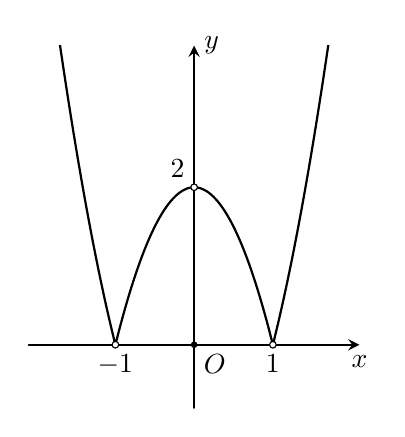
\begin{tikzpicture}[line cap=round, line join=round, >=stealth, scale=1]
				% Define plotting domain and bounding box
				\def\xmin{-2.1} \def\xmax{2.1}
				\def\ymin{-0.8} \def\ymax{3.8}
				
				% Scope to clip the curve safely within bounds
				\begin{scope}
					\clip (\xmin,\ymin) rectangle (\xmax,\ymax);
					
					% Graph of f(x) = 2*|x^2 - 1|
					\draw[black, thick, smooth, samples=200, domain=\xmin:\xmax]
					plot(\x, {2*abs((\x)^2 - 1)});
				\end{scope}
				
				% Draw Coordinate Axes (drawn on top of the curve)
				\draw[->, thick] (\xmin,0) -- (\xmax,0) node[below]{$x$};
				\draw[->, thick] (0,\ymin) -- (0,\ymax) node[right]{$y$};
				
				% Mark key points with small open circles as shown in the image
				\draw[fill=white] (-1,0) circle (1.2pt);
				\draw[fill=white] (1,0) circle (1.2pt);
				\draw[fill=white] (0,2) circle (1.2pt);
				\fill (0,0) circle (1.2pt);
				
				% Labels for key points and origin
				\node[below right] at (0,0) {$O$};
				\node[below] at (-1,0) {$-1$};
				\node[below] at (1,0) {$1$};
				\node[above left] at (0,2) {$2$};
			\end{tikzpicture}
			%		\end{center}
	\end{minipage}
	\begin{traloi}
		\dapan{Đ,S,Đ,S}
	\end{traloi}
\end{baitap}

\begin{baitap}
	%	\textbf{Câu 4.} 
	Cho hàm số $y=f(x)$ xác định và liên tục trên khoảng $(-3; 2)$ có $\lim\limits_{x \to (-3)^+} f(x) = -5$, $\lim\limits_{x \to 2^-} f(x) = 3$ và có bảng biến thiên như sau:
	
	\begin{minipage}{0.55\textwidth}
		\begin{enumerate}
			\item Hàm số không có GTNN trên khoảng $(-3; 2)$.
			\item Giá trị cực đại của hàm số bằng $0$.
			\item GTLN của hàm số trên khoảng $(-3; 2)$ bằng $0$.
			\item Giá trị cực tiểu của hàm số bằng $-2$.
		\end{enumerate}
	\end{minipage}	
	\begin{minipage}{0.45\textwidth}
		\begin{center}
			
\begin{tikzpicture}
				\tkzTabInit[lgt=1.2, espcl=2]{
					$x$/1,
					$y'$/1,
					$y$/1.5
				}{
					$-3$,
					$-1$,
					$1$,
					$2$
				}
				\tkzTabLine{,+,z,-,z,+,}
				\tkzTabVar{-/$-5$, +/$0$, -/$-2$, +/$3$}
			\end{tikzpicture}
		\end{center}
	\end{minipage}
	\begin{traloi}
		\dapan{Đ,Đ,S,Đ}
	\end{traloi}
\end{baitap}

\begin{baitap}
	%	\textbf{Câu 1.} Lê thánh tông 2025-2026
	Một công ty sản xuất một loại sản phẩm. Nếu có $x$ sản phẩm được bán ra thì hàm giá bán trên mỗi sản phẩm là $q(x) = 10000 - 250x$ (nghìn đồng), với $0 < x < 40$. Gọi $f(x)$ là hàm doanh thu của công ty (đơn vị: nghìn đồng). Xem $y = f(x)$ là một hàm số xác định trên khoảng $(0; 40)$. 
	\begin{enumerate}
		\item $f(x) = x \cdot q(x)$.
		\item $f'(x) = -500x + 10000$.
		\item Phương trình $f'(x) = 0$ có nghiệm là $x = 2$.
		\item Doanh thu lớn nhất của công ty bằng $100$ triệu đồng.
	\end{enumerate}
	\begin{traloi}
		\dapan{Đ,Đ,S,Đ} 
		
		Dưới đây là lời giải chi tiết và đánh giá tính đúng/sai cho từng phát biểu:
		\begin{enumerate}
			\item ĐÚNG. Giải thích: Doanh thu $f(x)$ được tính bằng số lượng sản phẩm bán ra nhân với giá bán trên mỗi sản phẩm:$$f(x) = x \cdot q(x) = x(10000 - 250x) \text{ (nghìn đồng)}$$
			\item ĐÚNG. Giải thích: Từ $f(x) = -250x^2 + 10000x$, tính đạo hàm ta được:$$f'(x) = (-250x^2 + 10000x)' = -500x + 10000$$
			\item SAI. Giải thích: Giải phương trình $f'(x) = 0$:$$-500x + 10000 = 0 \iff 500x = 10000 \iff x = 20$$Nghiệm của phương trình là $x = 20$ (thỏa mãn $0 < x < 40$), không phải $x = 2$.
			\item ĐÚNG. Giải thích: Vì $f''(x) = -500 < 0$ nên hàm số $f(x)$ đạt giá trị lớn nhất tại điểm tới hạn $x = 20$.Giá trị doanh thu lớn nhất là:$$f(20) = 20 \cdot (10000 - 250 \cdot 20) = 20 \cdot 5000 = 100000 \text{ (nghìn đồng)}$$Đổi đơn vị: 100 000 nghìn đồng = 100 000 000 đồng = 100 triệu đồng.
		\end{enumerate}
	\end{traloi}
\end{baitap}


\subsubsection*{Phần III. Thí sinh trả lời từ câu 1 đến câu 6 (không làm tròn các phép tính trung gian trong các câu từ 1 đến câu 6).}
\setcounter{bt}{0}
\begin{baitap}
	%	\textbf{Câu 1.} 
	Cho hàm số $y=f(x)$ liên tục trên đoạn $[-1; 3]$ và có đồ thị như hình vẽ bên dưới. Gọi $M, m$ lần lượt là giá trị lớn nhất và giá trị nhỏ nhất của hàm số đã cho trên đoạn $[-1; 3]$. Tính $M - m$.
	
	\begin{center}
		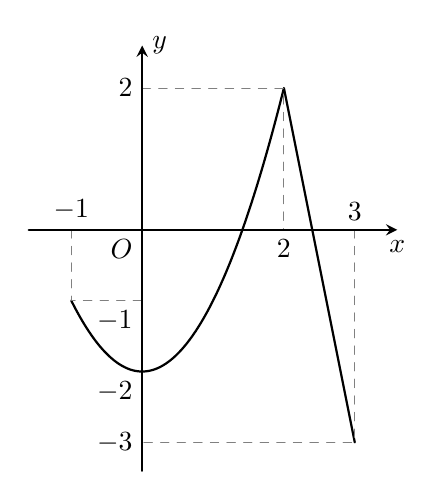
\begin{tikzpicture}[line cap=round, line join=round, >=stealth, scale=.9]
			% Define window bounds
			\def\xmin{-1.6} \def\xmax{3.6}
			\def\ymin{-3.4} \def\ymax{2.6}
			
			% Scope to clip elements safely within bounding box
			\begin{scope}
				\clip (\xmin,\ymin) rectangle (\xmax,\ymax);
				
				% Part 1: Parabola segment from x = -1 to x = 2
				% Passes through (-1, -1), min around (0, -1.8), and reaches (2, 2)
				% Curve fitting: y = 0.65*x^2 + 0.35*x - 1.3
				\draw[black, thick, smooth, samples=100, domain=-1:2]
				plot(\x, {(\x)^2  - 2});
				
				% Part 2: Line segment from (2, 2) to (3, -3)
				\draw[black, thick] (2,2) -- (3,-3);
			\end{scope}
			
			% Dashed projection lines for key points
			% Point (-1, -1)
			\draw[dashed, gray, thin] (-1,0) -- (-1,-1) -- (0,-1);
			
			% Peak (2, 2)
			\draw[dashed, gray, thin] (0,2) -- (2,2) -- (2,0);
			
			% Endpoint (3, -3)
			\draw[dashed, gray, thin] (3,0) -- (3,-3) -- (0,-3);
			
			% Draw Coordinate Axes
			\draw[->, thick] (\xmin,0) -- (\xmax,0) node[below]{$x$};
			\draw[->, thick] (0,\ymin) -- (0,\ymax) node[right]{$y$};
			
			% Label Origin
			\node[below left] at (0,0) {$O$};
			
			% Labels on X-axis
			\node[above] at (-1,0) {$-1$};
			\node[below] at (2,0) {$2$};
			\node[above] at (3,0) {$3$};
			
			% Labels on Y-axis
			\node[left] at (0,2) {$2$};
			\node[below left] at (0,-1) {$-1$};
			\node[below left] at (0,-2) {$-2$};
			\node[left] at (0,-3) {$-3$};
		\end{tikzpicture}
	\end{center}
	\begin{traloi}
		\dapan{5}
	\end{traloi}
\end{baitap}

\begin{baitap}
	%	\textbf{Câu 2.} 
	Biết hàm số $y = x^3 - 3x^2 - 9x + 28$ đạt giá trị nhỏ nhất trên đoạn $[0; 4]$ tại $x_0$. Tính $P = x_0 + 2$.
	\begin{traloi}
		\dapan{5}
	\end{traloi}
\end{baitap}

\begin{baitap}
	%	\textbf{Câu 4.} 
	Tìm $m$ để hàm số $y = \dfrac{x - m}{mx + 1}$ có giá trị nhỏ nhất trên $[0; 1]$ bằng $-2$.
	\begin{traloi}
		\dapan{2} 
	\end{traloi}
\end{baitap}

\begin{baitap}
	%	\textbf{Câu 5.} 
	Một xưởng in có $8$ máy in, mỗi máy in được \num{3600} bản in trong một giờ. Chi phí để vận hành một máy in trong mỗi lần in là $50$ nghìn đồng. Chi phí cho $n$ máy in chạy trong một giờ là $10(6n + 10)$ nghìn đồng. Hỏi nếu in \num{50000} tờ quảng cáo thì phải sử dụng bao nhiêu máy in để được lãi nhiều nhất?
	\begin{traloi}
		\dapan{5}
	\end{traloi}
\end{baitap}

\begin{baitap}
	%	\textbf{Câu 6.} 
	Ông An muốn xây một cái bể chứa nước lớn dạng một khối hộp chữ nhật không nắp có thể tích bằng \SI{288}{\cubic\meter}. Đáy bể là hình chữ nhật có chiều dài gấp đôi chiều rộng, giá thuê nhân công để xây bể là \num{500000} đồng/\SI{}{\square\meter}. Nếu ông An biết xác định các kích thước của bể hợp lý thì chi phí thuê nhân công sẽ thấp nhất. Hỏi ông An trả chi phí thấp nhất để xây dựng bể đó là bao nhiêu? (Đơn vị: triệu đồng)
	\begin{traloi}
		\dapan{108}	
	\end{traloi}
\end{baitap}

\begin{baitap}
	Cho hàm số $y = f(x) = \dfrac{x^2 + x + 2}{x - 1}$. Gọi $M$ là giao điểm của đồ thị hàm số $y = f(x)$ với trục tung. Phương trình tiếp tuyến của đồ thị hàm số $y = f(x)$ tại điểm $M$ là $y = ax +b$ với $ a,b $ là các số nguyên. Tính giá trị của $ a+b.$
	\begin{traloi}
		\dapan{-5} Phương trình tiếp tuyến là $ y=-3x-2 $.
	\end{traloi}
\end{baitap}